%\begin{itemize}
%\item Ahmad Syafrizal Huda (1164062)
%\item Annisa Fathoroni (1164067)
%\item Puad Hamdani (1164084)
%\item Rahmi Roza (1164085)
%\item Tasya Wiendhyra (1164086)
%\end{itemize}

\section{Definisi Flask GET}
Flask merupakan microframework yang dibangun dengan menggunakan bahasa pemrograman Python. Flask digunakan untuk me-develop sebuah aplikasi web. Flask merupakan microframework yang artinya flask membuat sebuah pengerjaan aplikasi web menjadi mudah dan simple karena dapat menjalankan sebuah web hanya dengan menggunakan 1 file Python. Flask membuat susunan kerja yang ringan, dan mudah tetapi juga dapat dikembangkan dengan mudah. Setiap data memiliki akses dengan berbagai HTTP Method seperti GET (Menerima data dalam bentuk array atau object) \cite{gunawan2018aplikasi}.
\subsection{pengertian GET request pada Flask}
GET request merupakan cara termundah untuk mengambil data dari pengguna. GET request tidak boleh mengubah status server yang dapat mengakibatkan efek samping.  Maka dari itu pengguna harus dapat membuat request yang sama dan harus mendapatkan hasil yang sama juga secara berkala. Oleh karena itu, GET request sangat ideal untuk memungkinkan pengguna untuk membedakan atau menentukan publikasi mana untuk dilihat\cite{dwyer2016flask}
GET merupakan sebuah method yang digunakan untuk mengambil sebuah sumber yang di identifikasikan dengan mengambil sebuah URL yang akan menampilkan operasi READ. Dengan method GET dapat mendapatkan informasi tanpa harus mengupdate database yang ada.GET digunakan untuk melempar value agar diproses ke web server dan kemudian selanjutnya value itu diberikan ke sebuah variabel untuk diproses oleh server dari web yang ada \cite{alemu2014rest}.
\subsection{Istilah Flask GET}
Informasi yang dikirim dari form dengan metode GET dapat terlihat oleh semua orang (semua nama variabel dan nilai-nilai variabel ditampilkan di URL). GET juga memiliki batasan pada jumlah informasi untuk mengirim. pembatasan itu sekitar 2000 karakter. Namun, karena variabel ditampilkan di URL, ini memungkinkan untuk sebagai penunjuk halaman. Dan hal ini dapat berguna dalam beberapa kasus tertentu. GET dapat digunakan untuk mengirim data yang tidak bersifat sensitif.
Apabila data yang dikirim ke server berupa data umum dan biasanya untuk memperjelas data yang dimasukkan di form, Anda dapat menggunakan method GET, misalnya untuk form pencarian data, polling dan lainnya \cite{grinberg2018flask}.
\subsection{Mendapatkan masukan pengguna menggunakan HTTP GET}
Oleh karena itu, permintaan GET sangat ideal untuk memungkinkan pengguna kami menentukan publikasi mana untuk melihat. Mari kita memperluas proyek Headlines kami untuk menggabungkan memilih judul berdasarkan atas permintaan GET. Pertama, mari kita memodifikasi kode Python untuk melakukan hal berikut \cite{dwyer2016flask}:
\begin{itemize}
\item Impor konteks permintaan dari Flask
\item Hapus variabel URL dinamis
\item Periksa untuk melihat apakah pengguna telah memasukkan publikasi yang valid sebagai argumen GET
\item Lewati kueri pengguna dan publikasi ke templat
\end{itemize}
\subsection{Metode Flask GET}
Metode penyediaan perintah operasional untuk program  yang dikirimkan menggunakan protokol HTTP termasuk menyimpan program  di server; menghasilkan data meta di server, di mana data meta mencakup tabel pemetaan yang menghubungkan rentang waktu untuk program  ke rentang byte untuk program  mentransmisikan data meta dan tabel pemetaan ke klien yang terkait dengan server, menghasilkan dan mentransmisikan perintah GET HTTP dari klien  ke server sebagai fungsi dari perintah operasional yang diinginkan; dan memilih I-frame yang tepat di server dan mengirimkan I-frame ke klien sebagai tanggapan atas perintah HTTP GET \cite{xu2006method}.
\subsubsection{Elemen GET}
Elemen (HEAD, OPTIONS, GET) yang ditampilkan di peta URL adalah metode permintaan yang ditangani oleh rute. Spesifikasi HTTP mendefinisikan bahwa semua permintaan dikeluarkan dengan metode, yang biasanya menunjukkan tindakan apa yang diminta klien untuk dilakukan oleh server. Flask menempelkan metode ke setiap rute sehingga metode permintaan yang berbeda dikirim ke URL yang sama dapat ditangani oleh fungsi tampilan yang berbeda.
Metode HEAD dan OPTIONS dikelola secara otomatis oleh labu, sehingga dalam praktiknya dapat dikatakan bahwa dalam aplikasi ini tiga rute dalam peta URL dilampirkan ke metode GET, yang digunakan ketika klien ingin meminta informasi seperti web halaman. Secara default, rute Flask merespon permintaan GET. Namun, preferensi ini dapat diubah dengan menyediakan metode argumen untuk rute () dekorator\cite{grinberg2018flask}.
\subsubsection{Framework Cookbook}
Secara default, fungsi tampilan flask hanya mendukung permintaan GET. Untuk mendukung atau menangani jenis permintaan lainnya, harus secara khusus memberitahu rute () decorator tentang mode yang ingin dukung. Inilah yang dilakukan di dua terakhir metode untuk POST dan GET/POST. Untuk permintaan GET, objek permintaan akan mencari argument, yaitu request.args.get(), dan untuk POST, itu akan mencari bentuk, yaitu request.from.get(). Selain itu, jika mencoba membuat permintaan GET ke metode yang hanya mendukung POST, permintaan akan gagal \cite{aggarwal2014flask}.
\subsubsection{Working with Views}
Fungsi tampilan Flask hanya mendukung permintaan GET. Hal yang sama berlaku dalam hal pandangan berbasis kelas. Untuk mendukung atau menangani jenis permintaan lainnya, harus secara khusus memberi tahu kelas, melalui metode atribut kelas yang disebut, tentang metode HTTP ingin mendukung. Untuk permintaan GET, objek permintaan akan mencari argumen, yaitu, request.args.get (), dan untuk POST, itu akan mencari bentuk, yaitu, request.form.get (). Jika mencoba membuat permintaan GET ke metode yang hanya mendukung POST, permintaan akan gagal dengan kesalahan HTTP 405. Hal yang sama berlaku untuk semua metode \cite{aggarwal2014flask}.
\subsection{Method and system for inserting POST data into the GET request to apply normal caching rules}
Metode dan sistem untuk cache konten yang diminta HTTP POST menggunakan aturan caching standar yang terkait dengan permintaan HTTP GET diungkapkan. Ketika permintaan POST diterima, itu diubah menjadi permintaan GET dengan tag identifikasi. Tag pengidentifikasi mencakup nilai indeks yang unik untuk permintaan POST dan didasarkan pada URL permintaan POST dan payload. Ketika permintaan POST belum ditemukan sebelum URL permintaan POST dan payload disimpan di penyimpanan data. Klien kemudian menerima tanggapan pengalihan termasuk permintaan GET dengan tag identifikasi yang digunakan untuk meminta data. Ketika permintaan GET berikutnya dengan tag identifikasi diterima, ditentukan jika konten yang diminta telah di-cache. Jika demikian, konten yang di-cache dikembalikan ke klien. Jika tidak, permintaan POST asli dibuat kembali dan dikirim ke server asal untuk mengambil konten. Konten yang dikembalikan dikirim ke klien dan di-cache menggunakan permintaan GET dengan tag pengenal \cite{sloat2009method}.
\subsection{Process Flow}
Permintaan GET diubah menjadi permintaan POST dan payload yang diambil sekarang dimasukkan sebagai badan permintaan POST baru ini. Permintaan POST ini kemudian dikirim ke server asal untuk mengambil konten yang diminta. Ketika server asal merespon, dua hal terjadi. Data respons dikirim kembali ke klien panggilan (blok 730). Pada saat yang sama, konten yang diterima disimpan (blok 725) \cite{sloat2009method}.
\subsection{Summary}
Menurut masih aspek lain dari penemuan ini, ketika permintaan GET dengan tag identifikasi diterima, ditentukan jika konten yang diminta telah di-cache. Jika demikian, konten yang di-cache dikembalikan ke klien. Jika tidak, permintaan POST asli dibuat kembali dan dikirim ke server asal untuk mengambil konten. Konten yang dikembalikan dikirim ke klien dan di-cache menggunakan permintaan GET dengan tag pengenal \cite{sloat2009method}.

\section{Implementasi Pada Flask GET}
\subsection{Sistem Terintegrasi Berbasis Ajax untuk Pengelolaan Data Bencana Alam di Indonesia}
Metode GET dan POST merupakan objek XHR yang sama bekerja sebagai standar HTTP request. Menggunakan salah satu, baik metode GET atau POST dapat digunakan untuk melakukan permintaan data dan menerima tanggapan dari server dengan format standar. Format standar yang dapat diterima dari server adalah XML, JSON (Javascript Object Notation), dan teks \cite{prasetyo2007sistem}.
\subsection{Sistem Terintegrasi Berbasis Ajax untuk Pengelolaan Data Bencana Alam di Indonesia}
Objek XHR (XMLHttpRequest) adalah inti dari Ajax angine. XHR merupakan objek yang memberikan kemampuan sebuah halaman untuk mendapatkan data (menggunakan metode GET) atau mengirim data (menggunakan metode POST) dari server yang prosesnya terjadi di belakang layar, itu berarti refresh browser tidak diperlukan sepanjang proses ini. Hal inilah yang menjadi factor kunci dalam memberikan kelebihan aplikasi kepada user. User tidak perlu mengetahui proses sehingga dapat focus dengan pekerjaan yang dilakukan \cite{prasetyo2007sistem}.
\subsection{Implementasi pengkodean sistem Python dengan versi 2.7.13.}
Implementasi pengkodean sistem, menggunakan Bahasa pemrograman Python dengan versi 2.7.13. Framework yang digunakan untuk sistem ini adalah Flask Micro-Framework. Adapun beberapa library yang mendukung sistem ini adalah:
\begin{enumerate}
\item Pandas
\item Matplotlib
\item Scikit-learn
\item Flask-CORS
\item Jupyter Notebook
\item Pymysql
\item Scipy
\end{enumerate}
Selain itu aplikasi juga dijalankan dalam server dan diatur oleh Apache Server dengan memanfaatkan mod wsgi. Database yang digunakan pada aplikasi ini adalah MySQL\cite{gunawan2018aplikasi}.
\subsection{REST API, Implementation with Flask-Python}
\subsubsection{Flask-SQLAlchemy}
Berikut ini adalah demonstrasi bagaimana sumber daya diwakili dalam aplikasi web.
Sumber daya ini diserialkan ke format JSON dari database SQLAlchemy obyek. Oleh karena itu, ini meningkatkan kinerja API dengan memungkinkan pengguna untuk mengonsumsi dengan mudah. Contoh pertama menunjukkan bagaimana merepresentasikan daftar sumber daya posting yang dibuat oleh pengguna tertentu yang diidentifikasi oleh idnya. Selain itu, representasi ini juga menunjukkan kemungkinan tautan (negara) yang dapat ditransfer dari node ini. Jadi, adokumentasi terpisah tidak boleh disiapkan sebagai panduan pengguna. Ini bisa dilakukan dengan mengirim permintaan GET ke server menggunakan URI http://localhost:5000/api/v1.0/ pengguna/2/posting \cite{alemu2014rest}.
\subsubsection{Perintah GET}
Perintah ini digunakan untuk melakukan semua HTTP permintaan. Sangat mudah untuk melakukan GET dari browser. Namun, untuk POST, PUT dan perintah DELETE request curl digunakan dari terminal. Karena itu, ikal perpustakaan harus diinstal pada komputer local untuk menjalankan semua perintah dokumen laporan ini. Selain itu, demontrasi ini menggunakan format JSON untuk dikirim dan menerima sumber daya melalui HTTP \cite{alemu2014rest}.
\subsection{Sistem Terintegrasi Berbasis Ajax untuk Pengelolaan Data Bencana Alam di Indonesia}
Pada model pertama sebuah static XML, JSON atau file teks yang berada pada domain yang sama di request oleh objek XHR melalui metode GET, lalu dikembalikan oleh server untuk ditangani oleh kode di sisi client yang melakukan permintaan. Semua ajax request dimulai dengan interaksi disisi client yang diatur oleh Javascript \cite{prasetyo2007sistem}.

\section{Contoh Flask GET}
\subsection{Request sederhana pada Flask Framework}
Berikut ini merupakan contoh skrip dari GET request :
\begin{figure}[ht]
\centerline{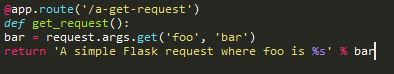
\includegraphics[width=1\textwidth]{figures/3FlaskGet.jpg}}
\caption{Method GET}
\label{labelgambar}
\end{figure}
Pada gambar\ref{labelgambar}Ini merupakan contoh sederhana dari apa GET request pada flask. Pada skrip ini hanya dilakukan pemeriksaan apakah query URL memiliki argumen yang disbut foo. apabila iya, maka akan menampilkan ini pada tanggapan, sedangkan jika tidak maka defaultnya adalah bar \cite{aggarwal2014flask}.
\subsection{Penggunaan Flask Get Request}
@hello.route('/')
@hello.route('/hello')
def helloworld():
user = request.args.get('user', 'Shalabh')
return rendertemplate('index.html', user=user)
Pada skrip diatas menggunakan metode get request, yang dimana jika ditemukan URL permintaan argumen, kita menggunakannya, dan jika tidak, kita menggunakan argumen default, Shalabh. Kemudian, nilai ini dilewatkan ke konteks template yang akan diberikan, yaitu index.html, dan template dihasilkan akan dituliskan\cite{aggarwal2014flask}.
\subsection{Tanpa GET}
Contoh ketika tidak menggunakan GET ketika melewati data yang sensitif seperti username dan password. Bisa juga pada saat Anda mengirimkan data dalam jumlah besar. GET hanya menggunakan sedikit karakter sehingga tidak dapat digunakan mengirim karakter yang besar \cite{gunawan2018aplikasi}.

\section{Keamanan Flask GET}
\subsection{deteksi serangan dos dengan http get}
Serangan DoS ke layanan Web disebut serangan banjir http-get dan ancamannya meningkat dari hari ke hari. Dalam jenis serangan ini, klien jahat mengirim sejumlah besar permintaan http-get ke server Web target secara otomatis. Karena permintaan http-get ini memiliki format yang sah dan dikirim melalui koneksi TCP normal, intrusion detection system (IDS) tidak dapat mendeteksi mereka. Dalam tulisan ini, kami mengusulkan teknik pendeteksian pendeteksian http-get berdasarkan analisis perilaku akses halaman. Kami mengusulkan dua algoritme deteksi, yang satu berfokus pada urutan penelusuran laman dan yang lainnya berfokus pada korelasi dengan waktu penelusuran ke ukuran informasi laman. Kami menerapkan teknik deteksi dan mengevaluasi tingkat deteksi serangan, yaitu, false positive dan false negative. Hasilnya menunjukkan bahwa teknik kami dapat mendeteksi serangan banjir http-get secara efektif \cite{yatagai2007detection}.
\subsection{Sistem Terintegrasi Berbasis Ajax untuk Pengelolaan Data Bencana Alam di Indonesia}
Pengiriman data ke Database-Enable XHR. Proses ini dimulai dengan sebuah XHR GET atau POST ke semua Bahasa sisi server. Sesudah server menerima permintaan, server memparsing XML atau nilai yang dikirim oleh XHR dan mengupdate database. Model request ini berdasarkan pada interaksi user, tanpa me-refresh browser. Pengiriman data ke database-enable XHR memberikan kemampuan penuh dalam mengontrol database melalui XHR \cite{prasetyo2007sistem}

\section{Kelebihan Metode GET pada Flask}
Berikut ini merupakan keuntungan dari Flask GET \cite{lokhande2015efficient}:
\begin{enumerate}
\item Sederhana, data mudah diedit.
\item Mudah untuk kembali ke halaman sebelumnya, misalnya dengan klik tombol back pada browser.
\item Dapat direfresh dengan mudah dan juga dapat di share apabila diperlukan.
\end{enumerate}
\subsection{Kegunaan Flask Method GET}
Pada tabel \ref{table:contoh} merupakan kegunaan daripada Flask pada Method GET \cite{grinberg2018flask}.
\begin{table}[h]
\begin{tabular}{|c|c|}
\hline
Macam Bentuk GET&Kegunaan\\
\hline
History&Parameter/nilai tersimpan dibrowser\\
&dan bisa diakses ulang karena nilai\\
&menjadi kesatuan URL.\\
Bookmark&Parameter bisa dibookmark\\
Parameters&Hanya bisa mengirimkan parameter\\
&melalui URL\\
Kecurangan data&Lebih terbuka karena data terlihat\\
Keamanan&Dengan jelas bisa ketahui data apa \\
&saja yang dikirim\\
Penggunaan&Digunakan lebih untuk keperluan \\
&mengambil data\\
\hline
\end{tabular}
\label{table:contoh}
\end{table}




